\documentclass[UTF8]{ctexart}
\usepackage{graphicx} % Required for inserting images
\usepackage{amsmath,amssymb,amsthm}
\usepackage{physics}
\usepackage{graphicx,float}
\graphicspath{{images/}}
\usepackage[none]{hyphenat}
\usepackage{blindtext}
\usepackage{parskip}
\usepackage[letterpaper,top=3cm, left= 3cm,bottom=3cm]{geometry}
\usepackage{subcaption}
\numberwithin{equation}{section}

\begin{document}
\section{洛伦兹变换}
在本题中,你将重走爱因斯坦的道路,推导狭义相对论中的时空变换(又称洛伦兹变换),并由此推导一些有意思的结论。
\subsection{准备工作}
\begin{enumerate}
    \item 在正式推导开始前,请简单阐述洛伦兹变换和牛顿力学中伽利略变换的区别
    \item 人类是如何意识到伽利略变换失效的?
\end{enumerate}
\subsection{伽利略变换}
在推导洛伦兹变换前,有必要先了解下伽利略变换。这有助于理解变换是什么,并提取些推导思路。

首先我们了解下什么是变换,考虑两个坐标系$S$系和$S'$系。伽利略变换提供了两个坐标系之间坐标$(x,y,z,t)$与$(x',y',z',t')$的转换公式。

请你推导经典理论中的伽利略变换。

提示:考虑两个坐标轴平行的参考系,,在$t = 0$时,两坐标系原点重合,$S'$系相对$S$系有一个朝$+x$方向的速度$v$。

\subsection{洛伦兹变换}
推导完伽利略变换后,下面你将推导洛伦兹变换。同样考虑两个坐标轴平行的参考系,在$t = 0$时,两坐标系原点重合,$S'$系相对$S$系有一个朝$+x$方向的速度$v$。
\begin{enumerate}
    \item 洛伦兹变换中,$y$和$y'$以及$z$和$z'$的关系是什么?
    \item 下面你要建立$(x,t)$和$(x',t')$的关系,请列出$x$与$x'$和$t'$以及$t$与$x'$和$t'$的关系,你应该列出一个四元一次方程(但是方程不一定有四条),这些方程的系数是我们想求的变换系数。
    
    提示:狭义相对论认为时间和空间都是线性变化的,换句话说$S$系中的坐标增量$\Delta x$正比于$S'$系中的坐标增量$\Delta x'$,对于时间也是同理。
\end{enumerate}

\newpage
\subsection{参考答案}
\subsubsection{准备工作}
\begin{enumerate}
    \item 伽利略变换假设的是绝对的时空,换句话说时间和空间在任意一个参考系下都是不变的,而洛伦兹变换没有这种特性。
    \item 迈克耳孙-莫雷实验指出了光速在任意参考系下都是不变的,伽利略变换中,光速不变是不成立的。
\end{enumerate}

\subsubsection{伽利略变换}
\begin{figure}[H]
    \centering
    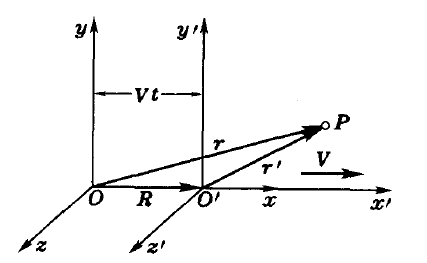
\includegraphics[width = 10cm]{Galileo.png}
    \caption{伽利略变换}
\end{figure}
很明显,$y$和$y'$坐标以及$z$和$z'$坐标是不改变的。同样,根据牛顿力学的时空观,两个坐标系下的时间坐标$t$和$t'$也相同。

因此变换的关键是求出$x$和$x'$的转换公式,不难看出$S'$系的原点在$S$系中的坐标为$vt$,因此可以得出$x' = x - vt$,至此,我们完整的推导了伽利略变换。
\[
\begin{cases}
    x' = x - vt\\
    y' = y\\
    z' = z\\
    t' = t\\
\end{cases}
\]

\newpage
\subsubsection{洛伦兹变换}
\begin{enumerate}
    \item $y' = y$,$z' = z$,因为在这两个坐标轴中没有相对运动。
    \item 
    \[
    \begin{cases}
    x = a_{11}x' + a_{12}t'\\
    t = a_{21} x' +a_{22}t'\\
    \end{cases}
    \]
    这样的假设保证了变换前后的线性时空
\end{enumerate}
\end{document}